% Provenance (never printed): see sources/outline_sources.md (Year 2: viscosity, density and
% volatiles of magmas; magma ascent; dykes, sills and plutons; contact aureoles).
% Curves from figdata/bachelor-2/magma.py (GRD 2008 viscosity, DensityX density, Moore 1998
% solubility data, erf sill cooling, Stefan solidification); exercise and problem values in
% the Book 4 scratch calculators calc/ch05.py and calc/ch05pb.py.
\chapter{Magmas and Their Emplacement}\label{ch:b2:magma-emplacement}

A basaltic melt at \qty{1200}{\celsius} flows with a viscosity of about
\qty{70}{Pa.s}: thick, but it pours. A dry rhyolitic melt at \qty{800}{\celsius}
has a viscosity near \qty{e11}{Pa.s}, and a block of it would take hours to sag
visibly under its own weight. Between the two lie ten orders of magnitude, more
than between water and the basalt, and most of the difference comes from two
things: the silica that links the melt into a network, and the temperature,
which is several hundred degrees lower in silicic \omterm{def:b2:magma-emplacement:magma}{magmas}. A few per cent of
dissolved water, which a rhyolitic \omterm{def:b2:magma-emplacement:magma}{magma} can hold at depth, brings its viscosity
down by a factor of \num{e5}, and loses it again as the \omterm{def:b2:magma-emplacement:magma}{magma} rises and the
water comes out as bubbles. These numbers decide whether a \omterm{def:b2:magma-emplacement:magma}{magma} reaches the
surface quietly, explodes, or freezes kilometres down as a \omterm{def:b2:magma-emplacement:bodies}{dyke}, a \omterm{def:b2:magma-emplacement:bodies}{sill} or a
\omterm{def:b2:magma-emplacement:bodies}{pluton}. This chapter treats a \omterm{def:b2:magma-emplacement:magma}{magma} as a material: its density, viscosity and
volatiles, the physics of its ascent through cracks and as blobs, the shapes it
takes when it stops, and the heat it gives to the rocks around it.
% ledger: grd08:model, grd08:range, moore98:melts

\begin{recall}
\textbf{Viscous flow} (physics books' Year 2 volume): in a Newtonian fluid of
viscosity $\eta$ the shear stress is $\eta$ times the velocity gradient; between
two parallel walls a pressure gradient drives a parabolic (plane Poiseuille)
profile; a sphere moving slowly through a viscous fluid feels the Stokes drag
$6\pi\eta a v$. \textbf{Heat conduction} (same volume): temperature obeys
$\partial T/\partial t = \kappa\,\partial^2T/\partial x^2$, with diffusivity $\kappa = k/(\rho
c)$, and a step of temperature spreads as an error function over a distance of
order $\sqrt{\kappa t}$. \textbf{Buoyancy} (physics books' Year 1 volume): a body
immersed in a denser fluid feels a net upward force equal to the weight of fluid
displaced minus its own. \textbf{Chemical equilibrium} (chemistry books): at
equilibrium the activities of products and reactants satisfy the law of mass
action with a constant $K$ that depends on temperature. From the Year 1 volume
of this series: the lithostatic pressure $p = \rho g z$ and the geotherm; from the
school volumes: mafic and felsic rocks, phenocrysts and porphyritic textures.
\end{recall}

\section{What a magma is}

\begin{definition}[Magma]\label{def:b2:magma-emplacement:magma}
A \emph{magma}\index{magma} is molten or partly molten rock beneath the surface: a
\emph{silicate melt}\index{silicate melt}, the liquid made mostly of silicon,
oxygen and metal cations, together with any crystals and gas bubbles it carries.
A \emph{crystal mush}\index{crystal mush} is a magma so rich in crystals that they
touch and form a framework: it cannot flow as a liquid, and its melt can only
move through the pores between crystals.
\end{definition}

The composition of the melt is given, as for rocks, in weight per cent of
oxides. Three melts serve as references throughout the chapter, all of them
studied in the laboratory: a tholeiitic basalt dredged from a mid-ocean ridge
(about \qty{51}{\percent} SiO$_2$, \qty{12}{\percent} iron oxide, \qty{7}{\percent}
MgO), an andesite (\qty{63}{\percent} SiO$_2$) and a rhyolite (\qty{78}{\percent}
SiO$_2$, \qty{8}{\percent} Na$_2$O $+$ K$_2$O and almost no iron or magnesium).
Their eruption temperatures differ as much as their compositions: basaltic
\omterm{def:b2:magma-emplacement:magma}{magmas} erupt at \qtyrange{1000}{1200}{\celsius} (lava streaming through a tube on
Kilauea has been measured near \qty{1200}{\celsius}), andesitic \omterm{def:b2:magma-emplacement:magma}{magmas} at
\qtyrange{800}{1000}{\celsius}, rhyolitic \omterm{def:b2:magma-emplacement:magma}{magmas} at \qtyrange{650}{800}{\celsius}.
A rhyolitic \omterm{def:b2:magma-emplacement:magma}{magma} is cooler because it is the residue of a long crystallisation
or the first melt of crustal rocks, both of which happen at low temperature
(\cref{ch:b2:magmatic-differentiation}).
% ledger: moore98:melts, tulane:magma-types, earle:kilauea-lava

The crystal content decides whether a \omterm{def:b2:magma-emplacement:magma}{magma} flows. Field and geochronological
studies of large granite bodies conclude that bulk magmatic flow needs a melt
fraction of at least \qtyrange{30}{50}{\percent} by volume; below that the
crystals are welded to their neighbours and the material deforms as a solid with
melt-filled pores. Much of the \omterm{def:b2:magma-emplacement:magma}{magma} stored in the crust is thought to sit in
that state, as a mush that becomes mobile again when hot \omterm{def:b2:magma-emplacement:magma}{magma} is added from
below.
% ledger: glazner04:tuolumne

\section{Density and viscosity}

\subsection{The density of a melt}

A \omterm{def:b2:magma-emplacement:magma}{silicate melt} has no crystal lattice, but its volume can still be built from
its components. Experiments on many melts show that each oxide contributes a
nearly fixed volume per mole, its partial molar volume, which changes slowly and
linearly with temperature and pressure; the volume of the melt is the sum of
these contributions. The table below gives the values used in this chapter.

\begin{table}[ht]
\centering\small
\begin{tabular}{lrrr}
\hline
Oxide & $\bar V_i$ (\unit{cm^3/mol}) & $\partial\bar V_i/\partial T$ (\num{e-3}\,\unit{cm^3/(mol.K)}) & $\partial\bar V_i/\partial p$ (\num{e-4}\,\unit{cm^3/(mol.bar)}) \\
\hline
SiO$_2$  & 26.86 & 0     & $-1.89$ \\
Al$_2$O$_3$ & 37.42 & 2.62 & $-2.26$ \\
FeO      & 12.68 & 3.69  & $-0.45$ \\
MgO      & 12.02 & 3.27  & $0.27$ \\
CaO      & 16.90 & 3.74  & $0.34$ \\
Na$_2$O  & 29.65 & 7.68  & $-2.40$ \\
K$_2$O   & 47.28 & 12.08 & $-6.75$ \\
H$_2$O   & 22.9  & 9.5   & $-3.20$ \\
\hline
\end{tabular}
\caption{Partial molar volumes of oxide components in \omterm{def:b2:magma-emplacement:magma}{silicate melts} at
\qty{1}{bar}, with their temperature and pressure derivatives. Reference
temperature \qty{1773}{K} (FeO \qty{1723}{K}, H$_2$O \qty{1273}{K}). Data:
compilation of the DensityX program (Iacovino and Till, 2019).}
\label{tab:b2:magma-emplacement:volumes}
\end{table}
% ledger: densityx:volumes

\begin{proposition}[Density of a silicate melt]\label{prop:b2:magma-emplacement:density}
Let a melt contain oxide components $i$ with mole fractions $X_i$, molar masses
$M_i$ and partial molar volumes $\bar V_i(T, p) = \bar V_i^{\circ} + (\partial\bar
V_i/\partial T)(T - T_{\mathrm{ref}}) + (\partial\bar V_i/\partial p)(p - p_{\mathrm{ref}})$.
If the components mix ideally in volume,
\[
\rho = \frac{\sum_i X_i M_i}{\sum_i X_i \bar V_i(T,p)}.
\]
\end{proposition}

\begin{proof}
One mole of melt contains $X_i$ moles of component $i$, of mass $X_iM_i$. Ideal
mixing in volume means that each mole of component $i$ adds the volume $\bar V_i$
whatever the others are, so the mole of melt occupies $\sum_i X_i\bar V_i$. The
density is the ratio of the two.
\end{proof}

Water has a molar mass of only \qty{18}{g/mol} but a partial molar volume of
\qty{22.9}{cm^3/mol}, close to that of silica: it lowers the density of a melt
strongly. Applied to the three reference melts, the proposition gives
\qty{2730}{kg/m^3} for the basalt at \qty{1200}{\celsius}, \qty{2480}{kg/m^3} for
the andesite at \qty{1000}{\celsius} and \qty{2340}{kg/m^3} for the dry rhyolite
at \qty{850}{\celsius}; one per cent of dissolved water takes about
\qty{70}{kg/m^3} off the basalt, as much as several hundred degrees of heating.
A basaltic melt is therefore lighter than the mantle peridotite it comes from
(about \qty{3380}{kg/m^3} below the crust in the reference Earth model) and a
little lighter than the lower crust of that model (\qty{2900}{kg/m^3}), while a
rhyolitic melt is lighter even than its upper crust (\qty{2600}{kg/m^3}). This difference drives \omterm{def:b2:magma-emplacement:magma}{magmas}
upward.
% ledger: densityx:volumes, densityx:water, data:prem

\subsection{Viscosity}

The viscosity of a \omterm{def:b2:magma-emplacement:magma}{silicate melt} is set by the network of SiO$_4$ tetrahedra
linked through shared oxygens: to flow, the melt must break and remake
silicon--oxygen bonds. Silica and alumina build the network; the cations of
magnesium, iron, calcium and the alkalis break it, and so does water, which
turns bridging oxygens into hydroxyl groups. Laboratory measurements on natural
melts cover more than fifteen orders of magnitude, from \qty{0.1}{Pa.s} to
\qty{e14}{Pa.s}, and they do not follow a simple Arrhenius law: the viscosity
rises faster than exponentially in $1/T$ as the melt cools towards its glass
transition.
% ledger: grd08:range

\begin{proposition}[Vogel--Fulcher--Tammann law]\label{prop:b2:magma-emplacement:vft}
The viscosity of a \omterm{def:b2:magma-emplacement:magma}{silicate melt} of fixed composition follows, to within a few
tenths of a logarithmic unit,
\[
\log_{10}\eta = A + \frac{B}{T - C},
\]
with $\eta$ in pascal seconds and $T$ in kelvins. For natural melts $A$ is close
to $-4.55$ whatever the composition; $B$ and $C$ (in kelvins) are linear
combinations of the mole percentages of the oxides, with a few products of them,
fitted to about \num{1800} measurements.
\end{proposition}
\admitted
% ledger: grd08:model, grd08:range

The figure below shows the law for the three reference melts and for the
rhyolite with dissolved water. At \qty{1200}{\celsius} the basalt has
$\eta \approx \qty{70}{Pa.s}$; the andesite at \qty{1000}{\celsius} is about
\qty{e6}{Pa.s}; the dry rhyolite at \qty{800}{\celsius} about $10^{10.9}$\,\unit{Pa.s}.
Four per cent of water brings the same rhyolite down to $10^{5.5}$\,\unit{Pa.s}, six
per cent to $10^{4.6}$\,\unit{Pa.s}. An independent equation fitted only to hydrous
granitic melts gives the same values to within half a logarithmic unit
(\cref{exo:b2:magma-emplacement:1}). The effect of water is largest at low temperature, where a few
tenths of a per cent change the viscosity by orders of magnitude.
% ledger: grd08:model, hd96:model, moore98:melts

\begin{omfigure}
\centering
\begin{tikzpicture}
\begin{axis}[omrecord, width=0.86\linewidth, height=6.4cm,
  xmin=600, xmax=1400, ymin=0, ymax=15,
  xlabel={temperature (\unit{\celsius})}, ylabel={$\log_{10}\eta$ (\unit{Pa.s})},
  legend pos=north east, legend style={font=\scriptsize},
  tick label style={font=\scriptsize}, label style={font=\small}]
\addplot[very thick, black, restrict x to domain=1000:1400] table[x=T_C, y=basalt] {figdata/out/bachelor-2-magma-visc.dat};
\addlegendentry{basalt, dry}
\addplot[very thick, brown, restrict x to domain=800:1300] table[x=T_C, y=andesite] {figdata/out/bachelor-2-magma-visc.dat};
\addlegendentry{andesite, dry}
\addplot[very thick, red!70!black, restrict x to domain=650:1100] table[x=T_C, y=rhyolite] {figdata/out/bachelor-2-magma-visc.dat};
\addlegendentry{rhyolite, dry}
\addplot[thick, red!70!black, dashed, restrict x to domain=650:1000] table[x=T_C, y=rhy2] {figdata/out/bachelor-2-magma-visc.dat};
\addlegendentry{rhyolite, 2 \% H$_2$O}
\addplot[thick, red!70!black, densely dotted, restrict x to domain=650:1000] table[x=T_C, y=rhy4] {figdata/out/bachelor-2-magma-visc.dat};
\addlegendentry{rhyolite, 4 \% H$_2$O}
\addplot[thick, red!70!black, dashdotted, restrict x to domain=650:1000] table[x=T_C, y=rhy6] {figdata/out/bachelor-2-magma-visc.dat};
\addlegendentry{rhyolite, 6 \% H$_2$O}
\end{axis}
\end{tikzpicture}
\par\smallskip{\small Viscosity of \omterm{def:b2:magma-emplacement:magma}{silicate melts} against temperature, from the
Vogel--Fulcher--Tammann law with the composition-dependent parameters of
Giordano, Russell and Dingwell (2008). Basalt: a mid-ocean ridge tholeiite;
andesite and rhyolite: laboratory reference melts (Moore and others, 1998). Each
curve is drawn over the temperatures at which such a \omterm{def:b2:magma-emplacement:magma}{magma} can be molten.}
\end{omfigure}
% ledger: grd08:model, moore98:melts

Crystals make a \omterm{def:b2:magma-emplacement:magma}{magma} stiffer still. A suspension of rigid particles resists
shear more than its liquid alone, because the liquid must flow around the
particles, and when the particles are crowded enough to touch they lock into a
framework.

\begin{proposition}[Einstein--Roscoe relation]\label{prop:b2:magma-emplacement:roscoe}
A suspension of a volume fraction $\phi$ of rigid spheres in a Newtonian liquid
of viscosity $\eta_{\ell}$ has the viscosity
\[
\eta = \eta_{\ell}\,(1 - R\phi)^{-2.5}, \qquad R = 1/\phi_m \approx 1.35,
\]
where $\phi_m$ is the maximum packing fraction, at which the suspension jams. For
small $\phi$ this reduces to Einstein's $\eta = \eta_{\ell}(1 + 2.5\phi)$.
\end{proposition}
\admitted
% ledger: kolz22:einstein-roscoe

Twenty per cent of crystals double the viscosity, forty per cent multiply it by
seven, sixty per cent by more than sixty (\cref{exo:b2:magma-emplacement:5}); in real \omterm{def:b2:magma-emplacement:magma}{magmas}, where the
crystals are elongated and of many sizes, the lock-up comes earlier, near the
\qtyrange{50}{70}{\percent} of crystals at which the field evidence places the
end of bulk flow.

\section{Volatiles}

\begin{definition}[Magmatic volatiles]\label{def:b2:magma-emplacement:volatiles}
A \emph{magmatic volatile}\index{magmatic volatile} is a component of a \omterm{def:b2:magma-emplacement:magma}{magma} that
is dissolved in the melt at depth and forms a separate gas phase at low
pressure: mainly water, then carbon dioxide, then sulfur species. \emph{Volatile
exsolution}\index{volatile exsolution} is the separation of a volatile from the
melt into bubbles of gas. The \emph{volatile saturation
pressure}\index{volatile saturation pressure} of a melt is the pressure below which
its dissolved volatiles exceed their solubility, so that a gas phase must form.
\end{definition}

Mafic \omterm{def:b2:magma-emplacement:magma}{magmas} typically carry \qtyrange{1}{3}{\percent} of volatiles by mass,
intermediate \omterm{def:b2:magma-emplacement:magma}{magmas} \qtyrange{3}{4}{\percent}, felsic \omterm{def:b2:magma-emplacement:magma}{magmas}
\qtyrange{4}{7}{\percent}, and the exsolution of \qtyrange{4}{6}{\percent} of
water drives most explosive eruptions. How much water a melt can hold depends
above all on pressure. The figure below shows measurements on basaltic and
rhyolitic melts held at a known water pressure until saturated, then quenched
to glass and analysed: the solubility rises steeply at low pressure and more
slowly at high pressure.
% ledger: earle:volatiles, moore98:arc-water, moore98:h2o

\begin{proposition}[Square-root law for water]\label{prop:b2:magma-emplacement:sqrt}
Suppose water dissolves in a \omterm{def:b2:magma-emplacement:magma}{silicate melt} mostly as hydroxyl groups, through
the reaction $\mathrm{H_2O\,(gas)} + \mathrm{O^{2-}\,(melt)} \rightleftharpoons
2\,\mathrm{OH^-\,(melt)}$, with the oxygen of the melt in large excess. Then, at
low water contents, the dissolved water is proportional to the square root of
the water pressure: $w \approx s\sqrt{p}$, with $s$ a constant of the melt and the
temperature.
\end{proposition}

\begin{proof}
The law of mass action gives $x_{\mathrm{OH}}^2 = K\,x_{\mathrm{O}}\,f$, where $f$ is
the fugacity of water (close to its pressure at moderate pressures) and the $x$
are mole fractions. The oxygen of the melt is in large excess, so
$x_{\mathrm{O}}$ stays nearly constant, and $x_{\mathrm{OH}} = \sqrt{Kx_{\mathrm{O}}}\,
\sqrt f$. Each dissolved water molecule makes two hydroxyls, so the dissolved
water is $x_{\mathrm{OH}}/2$, proportional to $\sqrt f$. At higher contents part
of the water dissolves as molecules, in proportion to $f$ itself, and the
solubility rises faster than the square root (\cref{exo:b2:magma-emplacement:10}).
\end{proof}

Fitted by least squares to the measurements, $w = s\sqrt p$ gives
$s = 0.34$ weight per cent per $\sqrt{\unit{MPa}}$ for the basalts and
$s = 0.44$ for the rhyolites; every measurement lies within one per cent of
water of its curve. The saturation pressure of a melt with $w$ per cent
of water is then $p_s = (w/s)^2$: \qty{129}{MPa} for a rhyolite with
\qty{5}{\percent} of water, about \qty{5}{km} down in the crust, but only
\qty{2}{MPa} for a basalt with \qty{0.5}{\percent}, a hundred metres or less.
% ledger: moore98:h2o

\begin{omfigure}
\centering
\begin{tikzpicture}
\begin{axis}[omrecord, width=0.8\linewidth, height=6cm,
  xmin=0, xmax=300, ymin=0, ymax=9,
  xlabel={water pressure (\unit{MPa})}, ylabel={dissolved H$_2$O (wt \%)},
  legend pos=south east, legend style={font=\scriptsize},
  tick label style={font=\scriptsize}, label style={font=\small}]
\addplot[very thick, red!70!black] table[x=P_MPa, y=rhyolite] {figdata/out/bachelor-2-magma-solub-fit.dat};
\addlegendentry{rhyolite, $0.44\sqrt p$}
\addplot[only marks, mark=*, mark size=2pt, red!70!black] table[x=P_MPa, y=w] {figdata/out/bachelor-2-magma-solub-rhyolite-data.dat};
\addlegendentry{rhyolite, measured}
\addplot[very thick, black] table[x=P_MPa, y=basalt] {figdata/out/bachelor-2-magma-solub-fit.dat};
\addlegendentry{basalt, $0.34\sqrt p$}
\addplot[only marks, mark=square*, mark size=2pt, black] table[x=P_MPa, y=w] {figdata/out/bachelor-2-magma-solub-basalt-data.dat};
\addlegendentry{basalt, measured}
\end{axis}
\end{tikzpicture}
\par\smallskip{\small Solubility of water in basaltic and rhyolitic melts at
\qtyrange{800}{1200}{\celsius} against the water pressure: measurements compiled
by Moore and others (1998), and least-squares square-root laws. At
\qty{100}{MPa}, about \qty{4}{km} deep in the crust, a rhyolite can hold
\qty{4.4}{\percent} of water, a basalt \qty{3.4}{\percent}.}
\end{omfigure}
% ledger: moore98:h2o

Carbon dioxide is far less soluble than water. It dissolves as molecules in
rhyolites and as carbonate groups in basalts, more in alkaline melts than in
tholeiites, and its solubility also rises with pressure. A \omterm{def:b2:magma-emplacement:magma}{magma} carrying both
gases therefore starts to exsolve deep, with a gas very rich in CO$_2$, and the
gas becomes richer in water as the \omterm{def:b2:magma-emplacement:magma}{magma} rises. Basalts erupted on the deep sea
floor contain vesicles of more than \qty{95}{\percent} CO$_2$, which required
saturation with CO$_2$ even under \qty{5}{km} of water. Estimates of the initial
CO$_2$ content of the parental basalts of Kilauea range from \qtyrange{0.2}{0.6}{\percent},
and melt inclusions trapped in their olivine crystals record saturation
pressures up to \qty{500}{MPa}.
% ledger: lowenstern01:co2, lowenstern01:basalts

Exsolved gas takes up a large volume. One per cent of water in a \omterm{def:b2:magma-emplacement:magma}{magma} at
\qty{900}{\celsius} occupies, as an ideal gas, about \qty{12}{\percent} of the
volume at \qty{100}{MPa}, \qty{57}{\percent} at \qty{10}{MPa} and more than
\qty{99}{\percent} at atmospheric pressure (\cref{exo:b2:magma-emplacement:7}). The bubbles lower the
density of the \omterm{def:b2:magma-emplacement:magma}{magma} further and drive it upward faster; in a viscous \omterm{def:b2:magma-emplacement:magma}{magma}
they cannot escape, and \cref{ch:b2:eruptive-styles} shows how they fragment it.

\section{Ascent}

A body of \omterm{def:b2:magma-emplacement:magma}{magma} less dense than its surroundings feels a buoyancy force of
$\Delta\rho\,g$ per unit volume, where $\Delta\rho$ is the density difference. It
can rise in two ways: through a crack it opens ahead of itself, or as a hot,
soft blob that pushes the surrounding rock aside.

\subsection{Dykes}

At depth the rock is under a large lithostatic pressure, but a crack filled
with \omterm{def:b2:magma-emplacement:magma}{magma} at a slightly higher pressure than the least principal stress can
open and lengthen at its tip. \omterm{def:b2:magma-emplacement:magma}{Magma} fills the crack as it grows, and the result
is a thin sheet of \omterm{def:b2:magma-emplacement:magma}{magma}, metres wide and kilometres long, that cuts its way
upward: a \omterm{def:b2:magma-emplacement:bodies}{dyke} in the making. The \omterm{def:b2:magma-emplacement:magma}{magma} then flows between two nearly parallel
walls.

\begin{proposition}[Flow of magma in a dyke]\label{prop:b2:magma-emplacement:poiseuille}
A Newtonian \omterm{def:b2:magma-emplacement:magma}{magma} of viscosity $\eta$ driven upward by a pressure gradient $G$
(for buoyant flow, $G = \Delta\rho\,g$) between two parallel walls a distance $w$
apart flows with the mean velocity
\[
\bar u = \frac{G w^2}{12\,\eta},
\]
and the volume flux per unit length of \omterm{def:b2:magma-emplacement:bodies}{dyke} is $q = \bar u w = G w^3/(12\eta)$.
\end{proposition}

\begin{proof}
In steady laminar flow the velocity profile across the \omterm{def:b2:magma-emplacement:bodies}{dyke} is the plane
Poiseuille parabola $u(x) = \frac{G}{2\eta}\left(\frac{w^2}{4} - x^2\right)$, for
$-w/2 \le x \le w/2$, which vanishes on both walls. Its mean is
$\bar u = \frac1w\int_{-w/2}^{w/2}u\,dx = \frac{G}{2\eta}\left(\frac{w^2}{4} -
\frac{w^2}{12}\right) = \frac{Gw^2}{12\eta}$.
\end{proof}

The cube of the width makes wide \omterm{def:b2:magma-emplacement:bodies}{dykes} far more efficient than narrow ones. A
basalt of \qty{100}{Pa.s} in a \omterm{def:b2:magma-emplacement:bodies}{dyke} \qty{1}{m} wide, with $\Delta\rho =
\qty{300}{kg/m^3}$, rises at about \qty{2.5}{m/s} and crosses \qty{10}{km} of
crust in an hour; a rhyolite of \qty{e6}{Pa.s} in the same \omterm{def:b2:magma-emplacement:bodies}{dyke} would take more
than a year, and would freeze on the way, so silicic \omterm{def:b2:magma-emplacement:magma}{magmas} need much wider
\omterm{def:b2:magma-emplacement:bodies}{dykes} (\cref{exo:b2:magma-emplacement:6}). The Reynolds number $\rho\bar u w/\eta$ of these flows
is small enough for them to stay laminar. Ascent rates estimated for \omterm{def:b2:magma-emplacement:magma}{magmas}
during eruptions separate effusive eruptions, below about \qty{0.1}{m/s}, from
explosive ones above it, with a transitional range from \qtyrange{0.005}{0.25}{m/s}
where both styles occur; kimberlites, which come from
depths beyond \qty{150}{km}, have been estimated at \qtyrange{0.1}{30}{m/s}, and
a diffusion study of one of them gives \qtyrange{0.02}{0.23}{m/s} averaged over
the last \qtyrange{80}{110}{km}, a journey of \numrange{5}{74} days.
% ledger: cassidy18:ascent, casetta23:kimberlite

\subsection{Diapirs}

\begin{definition}[Diapir, level of neutral buoyancy, stoping]\label{def:b2:magma-emplacement:ascent}
A \emph{diapir}\index{diapir} is a body of buoyant material, \omterm{def:b2:magma-emplacement:magma}{magma} or partly molten
rock, that rises through its surroundings by flowing them aside. The
\emph{level of neutral buoyancy}\index{level of neutral buoyancy} of a \omterm{def:b2:magma-emplacement:magma}{magma} is the
depth at which its density equals that of the surrounding rock: below it the
\omterm{def:b2:magma-emplacement:magma}{magma} is buoyant, above it it is denser than its surroundings. \emph{Magmatic
stoping}\index{magmatic stoping} is the detachment of blocks of the wall or roof
rock, which sink into the \omterm{def:b2:magma-emplacement:magma}{magma}; blocks that stay enclosed in the solidified
rock are xenoliths.
\end{definition}
% ledger: earle:intrusive-bodies

\begin{proposition}[Stokes ascent]\label{prop:b2:magma-emplacement:stokes}
A sphere of radius $a$ and density deficit $\Delta\rho$ rising slowly through a
Newtonian medium of viscosity $\eta$ reaches the terminal velocity
\[
v = \frac{2\,\Delta\rho\,g\,a^2}{9\,\eta}
\]
if it is rigid, and $1.5$ times this if it is a fluid of negligible viscosity.
\end{proposition}
\admitted

The rock around a \omterm{def:b2:magma-emplacement:ascent}{diapir} is not a fluid of \qty{100}{Pa.s} but a hot solid,
whose viscosity is many orders of magnitude higher than that of any melt: in the
crust, a sphere of \omterm{def:b2:magma-emplacement:magma}{magma} a kilometre across rises only millimetres a year, and
loses its heat long before it has risen far (\cref{exo:b2:magma-emplacement:9}). \omterm{def:b2:magma-emplacement:ascent}{Diapirs}
work where the surroundings are hot and soft, in the mantle and in the deep
roots of mountain belts, and where the buoyant material is a partly molten mass
kilometres across; the shallow crust is crossed by \omterm{def:b2:magma-emplacement:bodies}{dykes}.

\section{Emplacement}

Most \omterm{def:b2:magma-emplacement:magma}{magma} never reaches the surface. It stops where it is no longer buoyant,
or where it is blocked by a stronger layer, and spreads into a body whose shape
records how it made room for itself.

\begin{definition}[Intrusive bodies]\label{def:b2:magma-emplacement:bodies}
A \emph{pluton}\index{pluton} is any body of \omterm{def:b2:magma-emplacement:magma}{magma} that solidified within the
crust. A \emph{dyke}\index{dyke} is a sheet-like pluton that cuts across the
layering of its host rock (or any sheet if the host has no layering); a
\emph{sill}\index{sill} is a sheet-like pluton parallel to the layering. A
\emph{laccolith}\index{laccolith} is a sill that has thickened by pushing up the
overlying layers into a dome. A \emph{batholith}\index{batholith} is a large pluton,
or an assembly of plutons, with an exposed area of more than \qty{100}{km^2}.
\end{definition}
% ledger: earle:intrusive-bodies

\begin{omfigure}
\centering
\begin{tikzpicture}[x=1cm, y=1cm, font=\scriptsize]
% layered host
\fill[lith sandstone] (0,4.4) rectangle (12,5.4);
\fill[lith sandstone] (0,4.4) rectangle (12,5.4);
\fill[lith shale] (0,3.3) -- (0,4.4) -- (5.2,4.4) .. controls (5.7,4.95) and (7.0,4.95) .. (7.7,4.4)
  -- (12,4.4) -- (12,3.3) -- cycle;
\draw[thin] (0,4.4) -- (5.2,4.4) .. controls (5.7,4.95) and (7.0,4.95) .. (7.7,4.4) -- (12,4.4);
\fill[lith limestone] (0,2.2) rectangle (12,3.3);
\fill[lith sandstone] (0,0) rectangle (12,2.2);
\draw[thick] (0,0) rectangle (12,5.4);
% batholith at the bottom right
\fill[lith granite] (6.8,0) .. controls (7.2,1.6) and (8.4,2.2) .. (9.6,1.9)
  .. controls (10.6,1.7) and (11.2,1.3) .. (12,1.6) -- (12,0) -- cycle;
\draw[thick] (6.8,0) .. controls (7.2,1.6) and (8.4,2.2) .. (9.6,1.9)
  .. controls (10.6,1.7) and (11.2,1.3) .. (12,1.6);
% aureole around the batholith
\draw[densely dashed, orange!80!black, thick] (6.2,0) .. controls (6.6,2.2) and (8.4,2.8) .. (9.6,2.5)
  .. controls (10.6,2.3) and (11.3,2.0) .. (12,2.2);
% stoped blocks
\fill[lith limestone, draw=black] (8.4,1.0) rectangle (8.8,1.3);
\fill[lith sandstone, draw=black] (10.1,0.7) -- (10.5,0.8) -- (10.4,1.1) -- (10.0,1.0) -- cycle;
% feeder dyke from the bottom left, vertical
\fill[lith basalt] (2.0,0) rectangle (2.35,3.3);
\draw (2.0,0) -- (2.0,3.3) (2.35,0) -- (2.35,3.3);
% sill along shale/limestone contact
\fill[lith basalt] (2.0,3.15) rectangle (5.4,3.45);
\draw (2.0,3.15) -- (5.4,3.15) (2.35,3.45) -- (5.4,3.45);
% laccolith: lens pushing up the shale
\fill[lith basalt] (5.4,3.15) .. controls (5.6,3.95) and (6.6,4.05) .. (7.0,3.9)
  .. controls (7.3,3.8) and (7.4,3.4) .. (7.6,3.15) -- cycle;
\draw (5.4,3.45) .. controls (5.6,3.95) and (6.6,4.05) .. (7.0,3.9)
  .. controls (7.3,3.8) and (7.4,3.4) .. (7.6,3.15) -- (5.4,3.15);
% inclined dyke cutting to the surface from the laccolith
\fill[lith basalt] (6.6,3.95) -- (6.9,3.95) -- (7.6,5.4) -- (7.3,5.4) -- cycle;
% labels
\node[fill=white, fill opacity=0.8, text opacity=1, inner sep=1pt] at (1.2,1.4) {dyke};
\draw (1.6,1.4) -- (2.0,1.4);
\node[fill=white, fill opacity=0.8, text opacity=1, inner sep=1pt] at (3.6,2.7) {sill};
\draw (3.6,2.85) -- (3.6,3.15);
\node[fill=white, fill opacity=0.8, text opacity=1, inner sep=1pt] at (6.2,4.75) {laccolith};
\draw (6.2,4.6) -- (6.3,3.95);
\node[fill=white, fill opacity=0.8, text opacity=1, inner sep=1pt] at (9.6,0.5) {batholith};
\node[fill=white, fill opacity=0.8, text opacity=1, inner sep=1pt, align=center] at (10.6,3.0) {contact\\aureole};
\draw (10.6,2.7) -- (10.8,2.3);
\node[fill=white, fill opacity=0.8, text opacity=1, inner sep=1pt, align=left] at (5.0,1.0) {stoped\\blocks};
\draw (5.6,1.0) -- (8.35,1.15);
\end{tikzpicture}
\par\smallskip{\small Shapes of intrusive bodies in a layered host (schematic, not to
scale): a feeder \omterm{def:b2:magma-emplacement:bodies}{dyke} cutting across the layers, a \omterm{def:b2:magma-emplacement:bodies}{sill} along a bedding plane, a
\omterm{def:b2:magma-emplacement:bodies}{laccolith} doming the layers above it, a \omterm{def:b2:magma-emplacement:bodies}{dyke} cutting up to the surface, and a
\omterm{def:b2:magma-emplacement:bodies}{batholith} with blocks stoped from its roof and a \omterm{def:b2:magma-emplacement:aureole}{contact aureole}.}
\end{omfigure}

Where a \omterm{def:b2:magma-emplacement:magma}{magma} stops depends first on its density. In a crust whose density
increases with depth, a \omterm{def:b2:magma-emplacement:magma}{magma} rises to its \omterm{def:b2:magma-emplacement:ascent}{level of neutral buoyancy} and
spreads sideways there, as a \omterm{def:b2:magma-emplacement:bodies}{sill} or a lens; light sediments near the surface
are especially effective traps for dense basaltic \omterm{def:b2:magma-emplacement:magma}{magma}. A strong, stiff layer
can also stop a \omterm{def:b2:magma-emplacement:bodies}{dyke} and divert it along its base. The figure below shows the
principle.

\begin{omfigure}
\centering
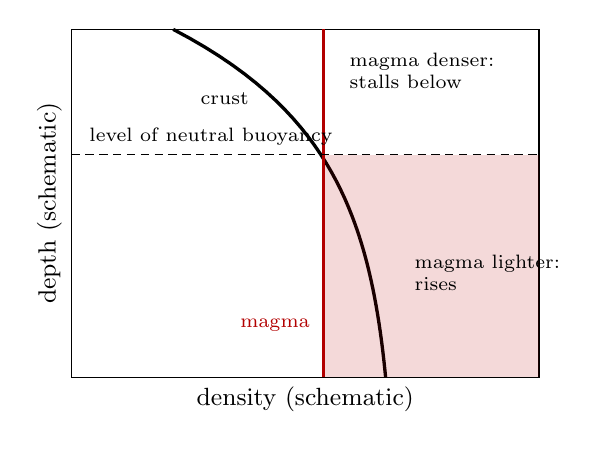
\begin{tikzpicture}[font=\scriptsize]
\begin{axis}[width=0.62\linewidth, height=6cm,
  xmin=0, xmax=1.15, ymin=0, ymax=1, y dir=reverse,
  xtick=\empty, ytick=\empty,
  xlabel={density (schematic)}, ylabel={depth (schematic)},
  label style={font=\small}, clip=false]
\addplot[very thick, black, domain=0:1, samples=40] ({0.25 + 0.55*(1 - exp(-3*x))}, {x});
\addplot[very thick, red!70!black] coordinates {(0.62,0) (0.62,1)};
\fill[red!70!black, opacity=0.15] (axis cs:0.62,0.36) rectangle (axis cs:1.15,1);
\draw[densely dashed] (axis cs:0,0.36) -- (axis cs:1.15,0.36);
\node[anchor=south west] at (axis cs:0.02,0.36) {level of neutral buoyancy};
\node[anchor=east, black] at (axis cs:0.46,0.20) {crust};
\node[anchor=east, red!70!black] at (axis cs:0.61,0.85) {magma};
\node[anchor=west, align=left] at (axis cs:0.82,0.70) {magma lighter:\\rises};
\node[anchor=west, align=left] at (axis cs:0.66,0.12) {magma denser:\\stalls below};
\end{axis}
\end{tikzpicture}
\par\smallskip{\small The \omterm{def:b2:magma-emplacement:ascent}{level of neutral buoyancy} (schematic). The density of
the crust increases with depth, by compaction of sediments and by the change to
denser rocks; a \omterm{def:b2:magma-emplacement:magma}{magma} of fixed density rises while it is lighter than its
surroundings (shaded) and spreads out where the two densities meet.}
\end{omfigure}

A \omterm{def:b2:magma-emplacement:bodies}{pluton} must make room for itself. It can lift its roof, as a \omterm{def:b2:magma-emplacement:bodies}{laccolith} does;
it can push its walls aside where they are soft; it can fill space opened by
faulting; and it can stope its roof, block by block. Large \omterm{def:b2:magma-emplacement:bodies}{plutons} were long
pictured as huge tanks of \omterm{def:b2:magma-emplacement:magma}{magma} emplaced at once. Dating has changed that
picture. The zircons of the Tuolumne Intrusive Suite, a granite \omterm{def:b2:magma-emplacement:bodies}{batholith} in
California, show that it was emplaced between \num{95} and \qty{85}{Ma}, oldest
at the margins and youngest at the centre, and one of its units alone over more
than \qty{3}{Myr}, between \qty{92.8}{Ma} and \qty{88.8}{Ma}. A single body of
\omterm{def:b2:magma-emplacement:magma}{magma} \qty{5}{km} thick and \qty{20}{km} wide emplaced at \qty{15}{km} depth would
have cooled below \qty{750}{\celsius}, where it is about half crystallised, in
about \num{500000}~years. Such \omterm{def:b2:magma-emplacement:bodies}{plutons} must have been assembled incrementally,
from many smaller intrusions such as sheets and \omterm{def:b2:magma-emplacement:bodies}{dykes}, over millions of years
(\cref{exo:b2:magma-emplacement:11}).
% ledger: glazner04:tuolumne

\begin{omfigure}
\centering
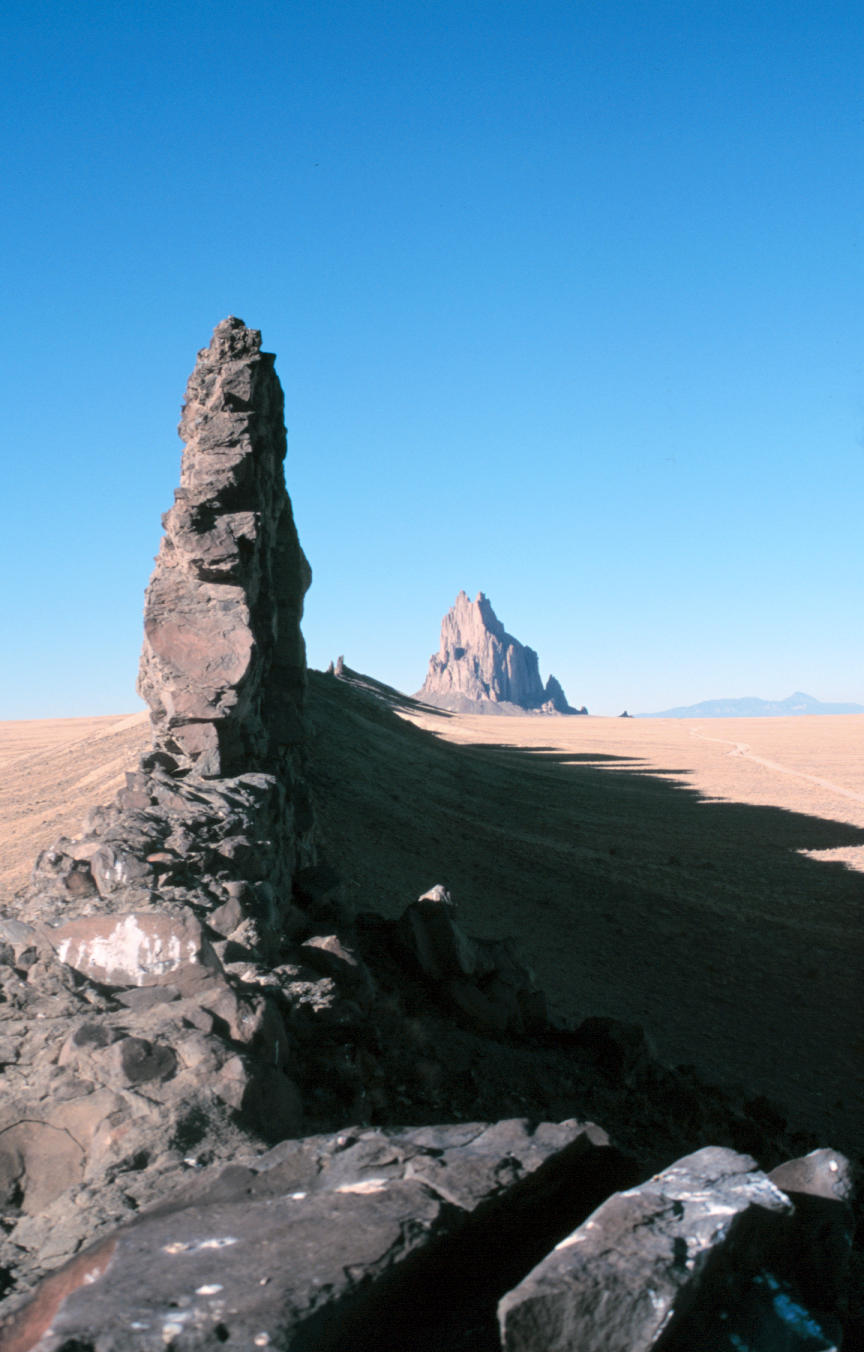
\includegraphics[width=0.3\linewidth]{images/book4/b2-shiprock-dyke.jpg}
\par\smallskip{\small A \omterm{def:b2:magma-emplacement:bodies}{dyke} near Shiprock, in the Navajo Volcanic Field
(New Mexico): the \omterm{def:b2:magma-emplacement:bodies}{dyke} rock resisted erosion better than the sandstone and shale
it cut, and now stands as a wall; in the distance, the volcanic neck from which
several such \omterm{def:b2:magma-emplacement:bodies}{dykes} radiate. Photograph: Dexter Perkins (CC0).}
\end{omfigure}

\section{Cooling and contact metamorphism}

An intrusion loses its heat by conduction into its host rocks. The simplest
model treats the intrusion and its host as one conducting medium of uniform
diffusivity $\kappa$: at time zero a sheet of thickness $b$ is at the intrusion
temperature $T_m$ and the host at $T_0$. The solution of the heat equation, with
$x$ measured from the middle of the sheet, is
\[
T(x,t) = T_0 + \frac{T_m - T_0}{2}\left[\operatorname{erf}\frac{b/2 - x}{2\sqrt{\kappa t}}
+ \operatorname{erf}\frac{b/2 + x}{2\sqrt{\kappa t}}\right].
\]
The figure below shows it for a \omterm{def:b2:magma-emplacement:bodies}{sill} \qty{100}{m} thick.
% ledger: delaney86b4:properties

\begin{proposition}[Contact temperature]\label{prop:b2:magma-emplacement:contact}
In this model, as long as $\sqrt{\kappa t}$ is small compared with $b$, the
temperature at the contact of the intrusion stays at the mean $(T_m + T_0)/2$ of
the intrusion and host temperatures.
\end{proposition}

\begin{proof}
At the contact $x = b/2$ the first error function is $\operatorname{erf}0 = 0$ and
the second is $\operatorname{erf}(b/(2\sqrt{\kappa t}))$, which is close to $1$ while
$b \gg 2\sqrt{\kappa t}$. Then $T = T_0 + (T_m - T_0)/2$.
\end{proof}

A basaltic \omterm{def:b2:magma-emplacement:bodies}{dyke} at \qty{1150}{\celsius} in rocks at \qty{50}{\celsius} thus heats
its contact to \qty{600}{\celsius}. The heat of crystallisation, typically
\qtyrange{700}{1000}{MJ/m^3}, keeps the \omterm{def:b2:magma-emplacement:magma}{magma} hot longer and raises this value:
with \qty{900}{MJ/m^3} released between \num{1150} and \qty{950}{\celsius} the same
model gives \qty{690}{\celsius}, while temperature-dependent conductivities and wet
host rocks lower both estimates by 50 to \qty{75}{\celsius}.
% ledger: delaney86b4:dike, delaney86b4:properties

\begin{omfigure}
\centering
\begin{tikzpicture}
\begin{axis}[omrecord, width=0.86\linewidth, height=6cm,
  xmin=-200, xmax=200, ymin=0, ymax=1200,
  xlabel={distance from the middle of the sill (\unit{m})},
  ylabel={temperature (\unit{\celsius})},
  legend pos=north east, legend style={font=\scriptsize},
  tick label style={font=\scriptsize}, label style={font=\small}]
\fill[gray!15] (axis cs:-50,0) rectangle (axis cs:50,1200);
\addplot[very thick, red!80!black] table[x=x_m, y=t1] {figdata/out/bachelor-2-magma-sill.dat};
\addlegendentry{1 year}
\addplot[very thick, orange!90!black] table[x=x_m, y=t2] {figdata/out/bachelor-2-magma-sill.dat};
\addlegendentry{10 years}
\addplot[very thick, blue!60!black] table[x=x_m, y=t3] {figdata/out/bachelor-2-magma-sill.dat};
\addlegendentry{50 years}
\addplot[very thick, black] table[x=x_m, y=t4] {figdata/out/bachelor-2-magma-sill.dat};
\addlegendentry{200 years}
\draw[densely dashed, gray] (axis cs:-200,625) -- (axis cs:200,625);
\node[font=\scriptsize, gray!40!black, anchor=south west] at (axis cs:-198,625) {$(T_m + T_0)/2$};
\node[font=\scriptsize, anchor=south] at (axis cs:0,20) {sill};
\end{axis}
\end{tikzpicture}
\par\smallskip{\small Conductive cooling of a \omterm{def:b2:magma-emplacement:bodies}{sill} \qty{100}{m} thick (shaded),
intruded at \qty{1150}{\celsius} into rock at \qty{100}{\celsius}, with
$\kappa = \qty{0.7e-6}{m^2/s}$ and no latent heat. The contact stays near
\qty{625}{\celsius} for decades while heat spreads into the host; after two
centuries the \omterm{def:b2:magma-emplacement:bodies}{sill} and its surroundings form one broad warm zone.}
\end{omfigure}
% ledger: delaney86b4:properties

The time scale of cooling is the time heat needs to diffuse across the
intrusion, of order $(b/2)^2/\kappa$: about \num{16} days for a \omterm{def:b2:magma-emplacement:bodies}{dyke}
\qty{2}{m} wide, a century for a \omterm{def:b2:magma-emplacement:bodies}{sill} \qty{100}{m} thick, a hundred thousand years
for a \omterm{def:b2:magma-emplacement:bodies}{pluton} of a few kilometres. The latent heat lengthens it, and so does the
need to solidify the \omterm{def:b2:magma-emplacement:magma}{magma} rather than merely cool it.

\begin{proposition}[Solidification of an intrusion]\label{prop:b2:magma-emplacement:stefan}
Let \omterm{def:b2:magma-emplacement:magma}{magma} at its solidification temperature $T_m$, with latent heat $L$ per unit
volume, fill the space $y > 0$ beside a host rock at $T_0$ occupying $y < 0$, both
of heat capacity $\rho c$ per unit volume and diffusivity $\kappa$. The
solidification front advances as $y_s = 2\lambda\sqrt{\kappa t}$, where $\lambda$
is the root of
\[
\frac{L\sqrt\pi}{\rho c\,(T_m - T_0)} = \frac{e^{-\lambda^2}}{\lambda\,(1 + \operatorname{erf}\lambda)},
\]
and the contact stays at $T_0 + (T_m - T_0)/(1 + \operatorname{erf}\lambda)$. A \omterm{def:b2:magma-emplacement:bodies}{sill}
of thickness $b$, solidifying from both walls, is solid after
$t = b^2/(16\lambda^2\kappa)$.
\end{proposition}

\begin{proof}
The \omterm{def:b2:magma-emplacement:magma}{magma} ahead of the front stays at $T_m$, so heat flows only in the solid
and the host, where we try $T = T_0 + (T_m - T_0)(1 + \operatorname{erf}\xi)/(1 +
\operatorname{erf}\lambda)$ with $\xi = y/(2\sqrt{\kappa t})$. Every function of $\xi$
of the form $\alpha + \beta\operatorname{erf}\xi$ solves the heat equation; this one
tends to $T_0$ far into the host ($\xi \to -\infty$) and equals $T_m$ on the front
$\xi = \lambda$. At $y = 0$ it gives the stated contact temperature. On the front,
the latent heat released by the advancing solid, $L\,dy_s/dt = L\lambda\sqrt{\kappa/t}$
per unit area and time, must be conducted away, $k\,\partial T/\partial y = k(T_m -
T_0)\,e^{-\lambda^2}/[(1 + \operatorname{erf}\lambda)\sqrt{\pi\kappa t}]$. Equating the
two and using $k = \rho c\kappa$ gives the equation for $\lambda$. Each wall of the
\omterm{def:b2:magma-emplacement:bodies}{sill} grows its own front, independently while the core stays at $T_m$; the two
fronts meet when $2\lambda\sqrt{\kappa t} = b/2$.
\end{proof}

With the latent heat of a basalt and a host at about \qty{100}{\celsius},
$\lambda$ is about $0.65$: a \omterm{def:b2:magma-emplacement:bodies}{sill} \qty{100}{m} thick solidifies in about
seventy years, and its contact stays near \qty{740}{\celsius} rather than
\qty{625}{\celsius} while it does. The weekend problem works through this case.
Because the time grows as the square of the thickness, a \omterm{def:b2:magma-emplacement:bodies}{sill} ten times thicker
takes a hundred times longer.

\begin{definition}[Contact aureole and its rocks]\label{def:b2:magma-emplacement:aureole}
A \emph{chilled margin}\index{chilled margin} is the fine-grained or glassy rim of an
intrusion, where the \omterm{def:b2:magma-emplacement:magma}{magma} cooled quickly against colder host rock. A
\emph{contact aureole}\index{contact aureole} is the zone of host rock around an
intrusion that was metamorphosed by its heat. \emph{Hornfels}\index{hornfels} is the
hard, fine-grained, non-foliated rock that mudstones and volcanic rocks become in
a contact aureole. \emph{Skarn}\index{skarn} is the rock formed where hot magmatic
fluids react with carbonate host rock, depositing calcium--iron--magnesium
silicates such as garnet and pyroxene, often with magnetite and metal sulfides.
\end{definition}
% ledger: earle:intrusive-bodies, earle:skarn

\omterm{def:b2:magma-emplacement:aureole}{Contact aureoles} range from a few centimetres around small \omterm{def:b2:magma-emplacement:bodies}{dykes} and \omterm{def:b2:magma-emplacement:bodies}{sills} to
several tens of metres around a large stock, and contact metamorphism spans
about \qty{300}{\celsius} to more than \qty{800}{\celsius}. A mudstone becomes a
\omterm{def:b2:magma-emplacement:aureole}{hornfels}, a limestone a marble, a sandstone a quartzite. A \omterm{def:b2:magma-emplacement:magma}{magma} emplaced deep
in rocks that are already hot makes almost no aureole: the width depends on the
size and temperature of the intrusion and on the temperature of its host, as
the cooling model predicts (\cref{exo:b2:magma-emplacement:12}). The minerals that grow in an aureole,
and what they say about temperature, belong to \cref{ch:b2:metamorphic-facies};
the metals that \omterm{def:b2:magma-emplacement:aureole}{skarns} concentrate to \cref{ch:b2:ore-deposits}.
% ledger: earle:skarn

\begin{inthefield}[Reading the contacts of a dyke]
\begin{minipage}[t]{0.6\linewidth}\vspace{0pt}
Where a \omterm{def:b2:magma-emplacement:bodies}{dyke} is exposed, a geologist first follows its contacts with the host
rock. A margin finer-grained or glassier than the centre of the \omterm{def:b2:magma-emplacement:bodies}{dyke} shows
that the \omterm{def:b2:magma-emplacement:magma}{magma} was chilled against cold rock; a \omterm{def:b2:magma-emplacement:bodies}{dyke} \qty{25}{cm} wide studied
on the coast of British Columbia has \omterm{def:b2:magma-emplacement:aureole}{chilled margins} \qty{2}{cm} thick. The host
rock is examined next to the contact for baking: a change of colour, a hardening,
new minerals that fade away from the \omterm{def:b2:magma-emplacement:bodies}{dyke}. The width of the baked zone and of
the \omterm{def:b2:magma-emplacement:aureole}{chilled margin}, measured against the width of the \omterm{def:b2:magma-emplacement:bodies}{dyke}, indicates how hot
the host was when the \omterm{def:b2:magma-emplacement:bodies}{dyke} arrived; a \omterm{def:b2:magma-emplacement:bodies}{dyke} with no \omterm{def:b2:magma-emplacement:aureole}{chilled margin} and no
aureole was intruded into rocks that were already hot. Samples are taken across
the \omterm{def:b2:magma-emplacement:bodies}{dyke}, from margin to centre, for the geochemistry of its melt and for the
size of its crystals.
\end{minipage}\hfill
\begin{minipage}[t]{0.36\linewidth}\vspace{0pt}
\centering
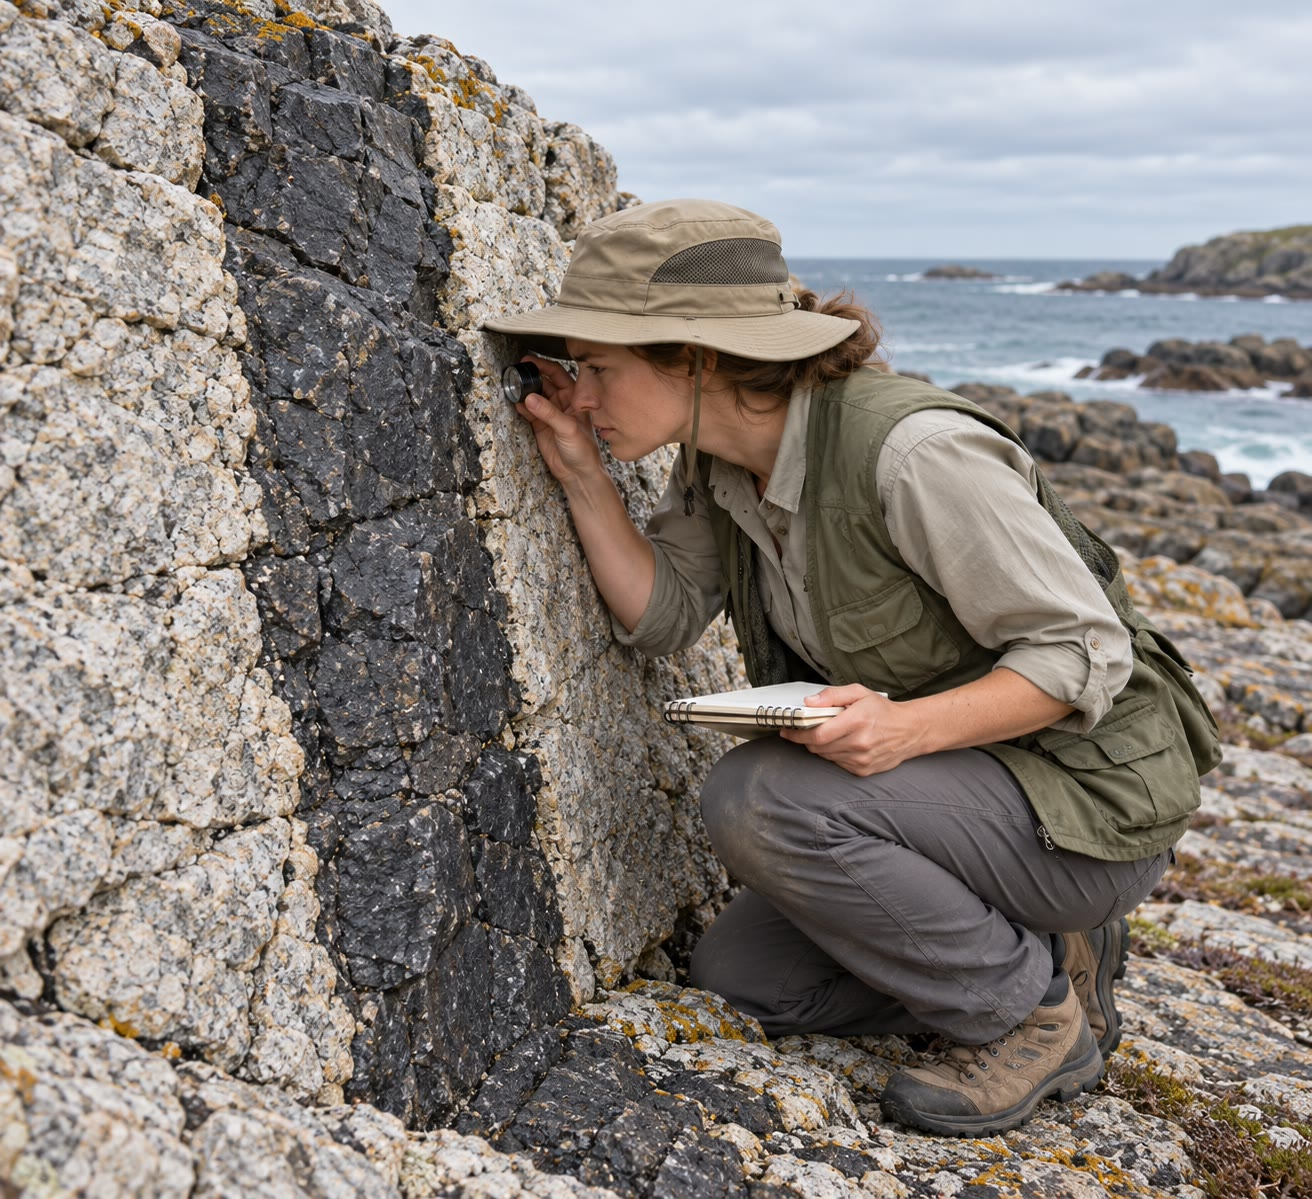
\includegraphics[width=\linewidth]{images/book4/ai/b2-dyke-contact.jpg}
\par\smallskip{\scriptsize A geologist examining the contact of a dark \omterm{def:b2:magma-emplacement:bodies}{dyke} with
pale host rock (AI-generated illustration).}
\end{minipage}
\end{inthefield}
% ledger: earle:intrusive-bodies

\section{Exercises}

\begin{exercise}[$\star$]\label{exo:b2:magma-emplacement:1}
For hydrous granitic melts, an equation fitted to measurements gives
$\log_{10}\eta = [-3.545 + 0.833\ln w] + [9601 - 2368\ln w]/\{T - [195.7 + 32.25\ln
w]\}$, with $\eta$ in \unit{Pa.s}, $w$ the water content in weight per cent and $T$
in kelvins. Compute $\log_{10}\eta$ at \qty{800}{\celsius} for $w = 1$ and $w = 4$,
and the factor by which the three extra per cent of water reduce the viscosity.
\end{exercise}
% ledger: hd96:model

\begin{exercise}[$\star$]\label{exo:b2:magma-emplacement:2}
With the square-root law, $s = 0.44$ for a rhyolite and $s = 0.34$ for a basalt
(weight per cent per $\sqrt{\unit{MPa}}$), compute the saturation pressure of a
rhyolite with \qty{6}{\percent} of water and of a basalt with \qty{0.5}{\percent},
and the corresponding depths in a crust of density \qty{2600}{kg/m^3}
($g = \qty{9.81}{m/s^2}$).
\end{exercise}

\begin{exercise}[$\star$]\label{exo:b2:magma-emplacement:3}
Compute the contact temperature of a basaltic \omterm{def:b2:magma-emplacement:bodies}{dyke} at \qty{1150}{\celsius}
intruded into rocks at \qty{50}{\celsius}, then into rocks at
\qty{400}{\celsius}. Which of the two \omterm{def:b2:magma-emplacement:bodies}{dykes} will have the wider \omterm{def:b2:magma-emplacement:aureole}{chilled margin}?
\end{exercise}

\begin{exercise}[$\star$]\label{exo:b2:magma-emplacement:4}
Name each body. (a) A sheet of dolerite \qty{30}{m} thick lying between two beds
of sandstone over \qty{20}{km}. (b) A vertical sheet of basalt \qty{2}{m} wide
cutting horizontal limestones. (c) A granite exposed over \qty{2000}{km^2},
made of a dozen units of different ages. (d) A lens of porphyry \qty{1}{km} across,
flat at its base, above which the beds are arched up. (e) A horizontal sheet
of basalt in a granite.
\end{exercise}

\begin{exercise}[$\star\star$]\label{exo:b2:magma-emplacement:5}
A basaltic melt has $\eta_{\ell} = \qty{100}{Pa.s}$. With the Einstein--Roscoe
relation ($R = 1.35$), compute the viscosity of the \omterm{def:b2:magma-emplacement:magma}{magma} with
\qty{5}{\percent}, \qty{20}{\percent}, \qty{40}{\percent} and \qty{60}{\percent} of
crystals, and compare the first with Einstein's dilute formula. At what crystal
fraction does the relation predict jamming?
\end{exercise}

\begin{exercise}[$\star\star$]\label{exo:b2:magma-emplacement:6}
\omterm{def:b2:magma-emplacement:magma}{Magma} of density \qty{300}{kg/m^3} less than its walls rises through a \omterm{def:b2:magma-emplacement:bodies}{dyke}.
(a) For a basalt ($\eta = \qty{100}{Pa.s}$, $\rho = \qty{2700}{kg/m^3}$) in a \omterm{def:b2:magma-emplacement:bodies}{dyke}
\qty{1}{m} wide, compute the mean velocity, the flux per metre of \omterm{def:b2:magma-emplacement:bodies}{dyke}, the
Reynolds number and the time to rise \qty{10}{km}. (b) Same time for a rhyolite of
\qty{e6}{Pa.s} in a \omterm{def:b2:magma-emplacement:bodies}{dyke} \qty{1}{m} wide, then \qty{10}{m} wide. (c) A \omterm{def:b2:magma-emplacement:bodies}{dyke}
\qty{1}{m} wide loses its heat in a time of order $(w/2)^2/\kappa$, with $\kappa =
\qty{1e-6}{m^2/s}$: which of the three ascents can succeed?
\end{exercise}

\begin{exercise}[$\star\star$]\label{exo:b2:magma-emplacement:7}
A \omterm{def:b2:magma-emplacement:magma}{magma} of density \qty{2400}{kg/m^3} at \qty{900}{\celsius} releases
\qty{1}{\percent} of its mass as water vapour. Treating the vapour as an ideal gas
($R = \qty{8.314}{J/(mol.K)}$, \qty{18.015}{g/mol}), compute the volume fraction of
gas in the \omterm{def:b2:magma-emplacement:magma}{magma} at \qty{100}{MPa}, \qty{10}{MPa} and \qty{0.1}{MPa}. Which of the
three values is the least reliable, and why?
\end{exercise}

\begin{exercise}[$\star\star$]\label{exo:b2:magma-emplacement:8}
In a basin, the density of the rocks increases with depth $z$ as $\rho(z) =
2300 + 60\,z$ (\unit{kg/m^3}, $z$ in \unit{km}) down to \qty{10}{km}. (a) Where is
the \omterm{def:b2:magma-emplacement:ascent}{level of neutral buoyancy} of a basaltic melt of \qty{2650}{kg/m^3}? (b) The
density model of this chapter shows that one per cent of dissolved water lowers
the density of a basaltic melt by about \qty{70}{kg/m^3}. Where does a melt with
one more per cent of water stop? (c) What is the buoyancy force per cubic metre
of the dry melt \qty{2}{km} below its \omterm{def:b2:magma-emplacement:ascent}{level of neutral buoyancy}?
\end{exercise}

\begin{exercise}[$\star\star$]\label{exo:b2:magma-emplacement:9}
Suppose a granitic \omterm{def:b2:magma-emplacement:ascent}{diapir} of radius \qty{1}{km} and density deficit
\qty{300}{kg/m^3} rises through lower crust of viscosity \qty{e19}{Pa.s}. Compute
its Stokes velocity (rigid sphere) in millimetres per year and the time to rise
\qty{10}{km}. Compare with the time scale $a^2/\kappa$ of its cooling, with $\kappa
= \qty{1e-6}{m^2/s}$. What do you conclude?
\end{exercise}

\begin{exercise}[$\star\star\star$]\label{exo:b2:magma-emplacement:10}
Water dissolves in a melt both as molecules, $x_m = K_1 f$, and as hydroxyl
groups, $x_{\mathrm{OH}}^2 = K_2 x_m$ (the oxygen of the melt in large excess), so
that the total dissolved water is $x = x_m + x_{\mathrm{OH}}/2$. (a) Express $x$ as a
function of $f$ and show that it behaves as $\sqrt f$ at low $f$ and as $f$ at
high $f$. (b) At what fugacity are the two forms of water equally abundant? (c)
With $K_1 = \qty{1e-4}{MPa^{-1}}$ and $K_2 = 0.2$, compute that fugacity, and the
share of water dissolved as hydroxyl at \qty{100}{MPa}.
\end{exercise}

\begin{exercise}[$\star\star\star$]\label{exo:b2:magma-emplacement:11}
A granite \omterm{def:b2:magma-emplacement:bodies}{pluton} of \qty{1000}{km^3} is assembled over \qty{4}{Myr}. (a) Compute
its mean \omterm{def:b2:magma-emplacement:magma}{magma} supply in \unit{km^3} per year and in \unit{m^3} per second. (b) A
single \omterm{def:b2:magma-emplacement:bodies}{dyke} \qty{1}{km} long and \qty{2}{m} wide, with a mean velocity of
\qty{0.8}{m/s}, feeds it: how long would the \omterm{def:b2:magma-emplacement:bodies}{dyke} take to deliver the whole
\omterm{def:b2:magma-emplacement:bodies}{pluton}? What fraction of the \qty{4}{Myr} is that? (c) If the \omterm{def:b2:magma-emplacement:bodies}{pluton} is built of
sheets \qty{20}{m} thick and \qty{10}{km} by \qty{10}{km} wide, how many sheets
are needed, and how much time separates two of them on average? (d) With
$\lambda = 0.65$ and $\kappa = \qty{0.7e-6}{m^2/s}$, how long does a sheet take to
solidify? Is the \omterm{def:b2:magma-emplacement:bodies}{pluton} ever a single large body of \omterm{def:b2:magma-emplacement:magma}{magma}?
\end{exercise}

\begin{exercise}[$\star\star\star$]\label{exo:b2:magma-emplacement:12}
Far from a thin \omterm{def:b2:magma-emplacement:bodies}{dyke} of width $b$ (at distances $x \gg b$), its heat acts as an
instantaneous plane source: $T - T_0 = (T_m - T_0)\,b\,e^{-x^2/(4\kappa
t)}/\sqrt{4\pi\kappa t}$. (a) Show that at distance $x$ the temperature is highest at
$t^* = x^2/(2\kappa)$, and that this highest rise is $\Delta T_{\max} = (T_m -
T_0)\,b/(x\sqrt{2\pi e})$. (b) For a \omterm{def:b2:magma-emplacement:bodies}{dyke} \qty{2}{m} wide with $T_m - T_0 =
\qty{1100}{K}$, at what distance does the rock warm by at most \qty{100}{K}, and
when ($\kappa = \qty{0.7e-6}{m^2/s}$)? (c) Why are the aureoles of thin \omterm{def:b2:magma-emplacement:bodies}{dykes} so
narrow?
\end{exercise}

\section{Problem: The sill under the plateau}

\begin{problem}[{Weekend problem --- following a basaltic magma from its feeder
dyke to a sill, its water, and the time the sill takes to solidify}]
\label{pb:b2:magma-emplacement:1}
Beneath an imaginary plateau, sediments (shale and sandstone) of mean density
\qty{2450}{kg/m^3} rest at \qty{3.0}{km} depth on a crystalline basement of
density \qty{2800}{kg/m^3}. A basaltic \omterm{def:b2:magma-emplacement:magma}{magma} rose from \qty{15}{km} through a \omterm{def:b2:magma-emplacement:bodies}{dyke}
\qty{2.0}{m} wide and spread along the base of the sediments as a dolerite \omterm{def:b2:magma-emplacement:bodies}{sill}
\qty{100}{m} thick. Data: intrusion temperature \qty{1150}{\celsius}; melt
viscosity law $\log_{10}\eta = -4.55 + 5510/(T - 611)$ ($T$ in kelvins); melt
density with its water \qty{2710}{kg/m^3}; \qty{20}{\percent} of crystals by volume
(Einstein--Roscoe, $R = 1.35$); dissolved water \qty{0.40}{\percent}, solubility
$s = 0.34$ per cent per $\sqrt{\unit{MPa}}$; temperature of the host at the \omterm{def:b2:magma-emplacement:bodies}{sill}
\qty{100}{\celsius}; $\kappa = \qty{0.7e-6}{m^2/s}$, $\rho c = \qty{2.5}{MJ/(m^3.K)}$,
latent heat \qty{900}{MJ/m^3}, the \omterm{def:b2:magma-emplacement:magma}{magma} being treated as solidifying at its
intrusion temperature; $g = \qty{9.81}{m/s^2}$; one year is \qty{3.156e7}{s}.

\medskip\noindent\textbf{Part I --- The magma.}
\begin{enumerate}
\item Compute $\log_{10}\eta$ and $\eta$ of the melt at \qty{1150}{\celsius}
(\qty{1423}{K}).
\item Same at \qty{1100}{\celsius}. By what factor does the viscosity change over
these \qty{50}{K}?
\item Compute the viscosity of the \omterm{def:b2:magma-emplacement:magma}{magma} with its crystals at
\qty{1150}{\celsius}.
\item At what crystal fraction would the Einstein--Roscoe relation make the
\omterm{def:b2:magma-emplacement:magma}{magma} jam? Compare with the field estimate of the end of bulk flow.
\item Compute the density difference between the \omterm{def:b2:magma-emplacement:magma}{magma} and the basement, and
between the \omterm{def:b2:magma-emplacement:magma}{magma} and the sediments.
\item Compute the lithostatic pressure at the level of the \omterm{def:b2:magma-emplacement:bodies}{sill}.
\end{enumerate}

\noindent\textbf{Part II --- Up the dyke.}
\begin{enumerate}[resume]
\item Compute the buoyant pressure gradient $\Delta\rho\,g$ that drives the \omterm{def:b2:magma-emplacement:magma}{magma}
through the basement.
\item Compute the mean velocity of the \omterm{def:b2:magma-emplacement:magma}{magma} in the \omterm{def:b2:magma-emplacement:bodies}{dyke}.
\item Compute the flux per metre of \omterm{def:b2:magma-emplacement:bodies}{dyke}, and the total flux if the \omterm{def:b2:magma-emplacement:bodies}{dyke} is
\qty{1.0}{km} long.
\item Compute the Reynolds number of the flow. Is it laminar?
\item How long does the \omterm{def:b2:magma-emplacement:magma}{magma} take to rise from \qty{15}{km} to \qty{3.0}{km}?
\item Compare with the time scale $(w/2)^2/\kappa$ over which the \omterm{def:b2:magma-emplacement:bodies}{dyke} loses its
heat. Can it stay open?
\item Explain why the \omterm{def:b2:magma-emplacement:magma}{magma} stopped at \qty{3.0}{km} and spread sideways, using
the chapter's vocabulary.
\end{enumerate}

\noindent\textbf{Part III --- The water.}
\begin{enumerate}[resume]
\item Compute the saturation pressure of the melt's water, and the depth in the
sediments where it is reached.
\item How much water could the melt hold at the level of the \omterm{def:b2:magma-emplacement:bodies}{sill}? Does the \omterm{def:b2:magma-emplacement:bodies}{sill}
\omterm{def:b2:magma-emplacement:magma}{magma} exsolve water?
\item Vesicles in the \omterm{def:b2:magma-emplacement:aureole}{chilled margin} of the \omterm{def:b2:magma-emplacement:bodies}{sill} contain mostly CO$_2$. Explain.
\item If all \qty{0.40}{\percent} of water came out at the surface, at
\qty{1150}{\celsius} and \qty{0.1}{MPa}, what volume fraction of the \omterm{def:b2:magma-emplacement:magma}{magma} would
the vapour occupy (ideal gas)?
\end{enumerate}

\noindent\textbf{Part IV --- Cooling and solidification.}
\begin{enumerate}[resume]
\item Ignoring latent heat, compute the contact temperature of the \omterm{def:b2:magma-emplacement:bodies}{sill}.
\item Ignoring latent heat, compute the temperature \qty{10}{m} above the top
contact \num{10}~years after the intrusion.
\item Same model: compute the temperature at the middle of the \omterm{def:b2:magma-emplacement:bodies}{sill} after
\num{10}~years and \num{50}~years.
\item Same model: \qty{80}{m} above the top contact, compute the temperature after
\num{300}, \num{363} and \num{420} years. Does the rock there ever reach
\qty{300}{\celsius}?
\item Compute $L\sqrt\pi/(\rho c\,(T_m - T_0))$ for the \omterm{def:b2:magma-emplacement:bodies}{sill}.
\item Evaluate $e^{-\lambda^2}/(\lambda(1 + \operatorname{erf}\lambda))$ for $\lambda = 0.64$,
$0.65$ and $0.66$ ($\operatorname{erf}0.64 = 0.6346$, $\operatorname{erf}0.65 = 0.6420$,
$\operatorname{erf}0.66 = 0.6494$), and give $\lambda$ to two decimals.
\item With latent heat, compute the contact temperature while the \omterm{def:b2:magma-emplacement:bodies}{sill}
solidifies. Why is it higher than in question 18?
\item Compute the time scale $(b/2)^2/\kappa$ in years.
\item Compute the time the \omterm{def:b2:magma-emplacement:bodies}{sill} takes to solidify, in years, the key number of
this problem, and explain why it is shorter than the time scale of the last
question even though latent heat must be removed.
\end{enumerate}
\end{problem}
% ledger: grd08:model, kolz22:einstein-roscoe, glazner04:tuolumne, moore98:h2o, lowenstern01:co2, delaney86b4:properties
